%%%%%%%%%% %%%%%%%%%% %%%%%%%%%% %%%%%%%%%% 
\section{Proposed Pipelined Computation Model}
%\fixme{1. Pipeline identification, 2. Resource Mapping, 3. Software optimizations, 4. Caching  IN THE SAME ORDER}
\label{sec:04Design}

% Text matter begin
%%%%%%%%%% %%%%%%%%%% %%%%%%%%%% %%%%%%%%%% 
%\subsection{Pipeline Design}
%Retrieval-Augmented Generation (RAG) has emerged as a powerful technique for leveraging external knowledge in language tasks. However, existing deployment strategies often fail to fully exploit the computational capabilities of edge platforms (such as desktops and mobile devices), leading to inefficient resource usage and suboptimal performance. 
% the model is not used in any ofht eother result fi\todo{use %figure~\ref{fig:pipeline_comparison_schematic} here. you can start with prior work limitations to reitrate the motivation for this section. }  

Here, we present the design choices behind a resource-aware framework for orchestrating the stages of RAG.
%In this section, we present the design choices behind a resource-aware framework that aims to address these limitations by carefully orchestrating the various stages of the RAG.
%workflow. 
%Our approach draws on a range of hardware and software optimizations, providing a flexible and efficient way to handle diverse workloads. 
%In subsequent sections, we describe the technical underpinnings of this design, detailing how each component contributes to higher throughput and lower latency. 




% \begin{figure}
% \centering
% 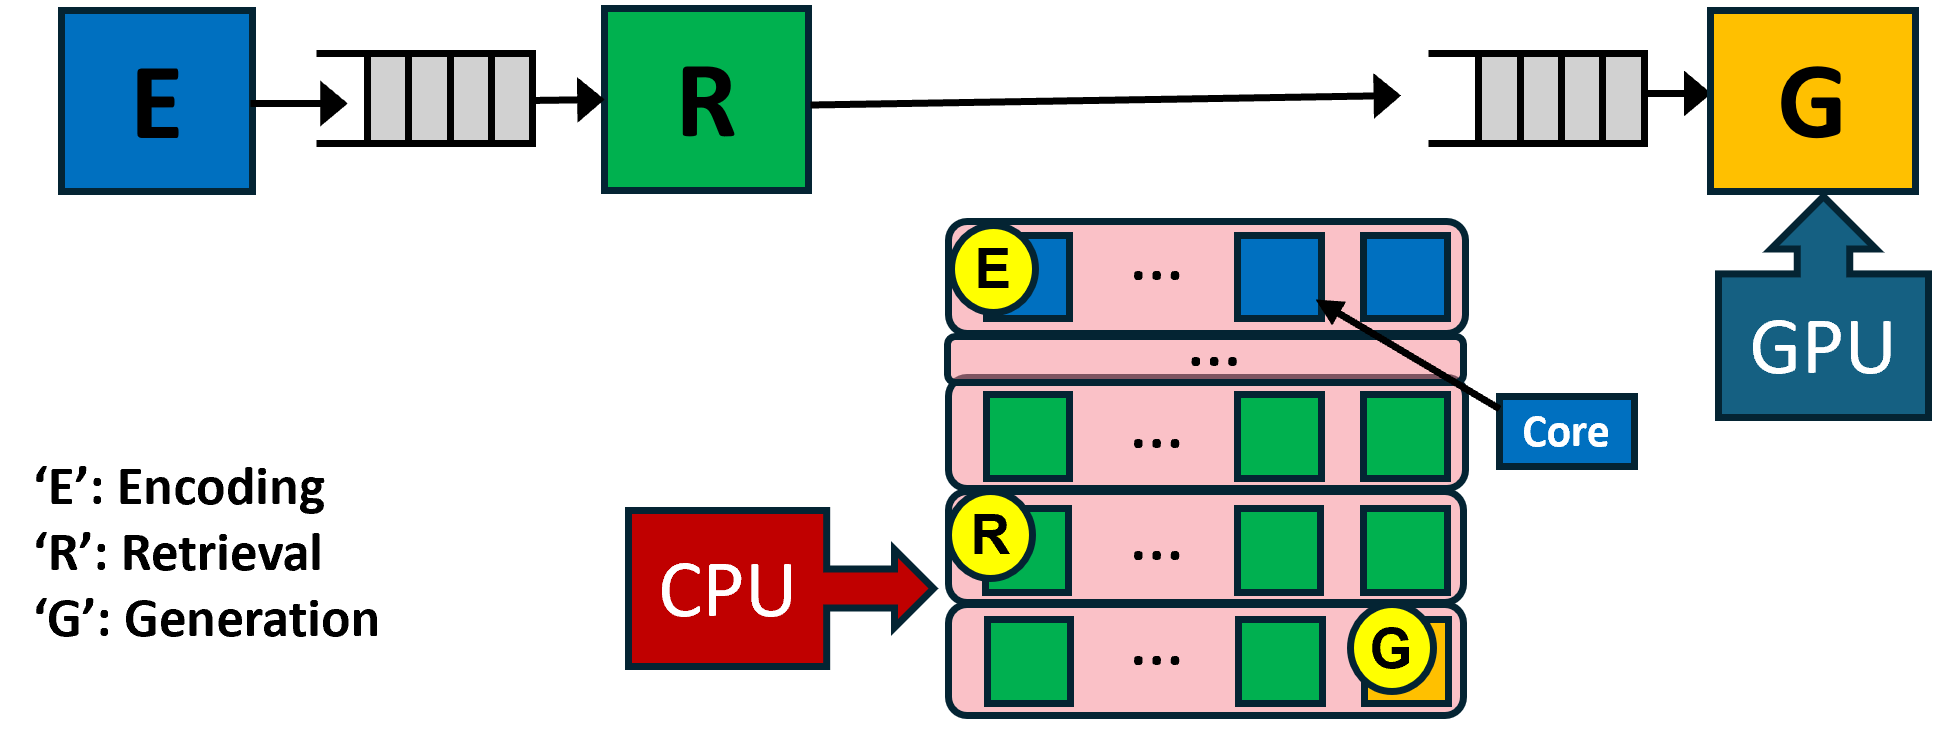
\includegraphics[width=1\linewidth]{diagrams/latency_oriented_pipeline.png}
% \caption{Proposed pipeline for latency-critical tasks having a minimum number of parallel workers in each stage to maximize the number of CPU cores provisioned per stage.}
% \label{fig:latency_oriented_pipeline} 
% \end{figure}


% \begin{figure}
% \centering
% 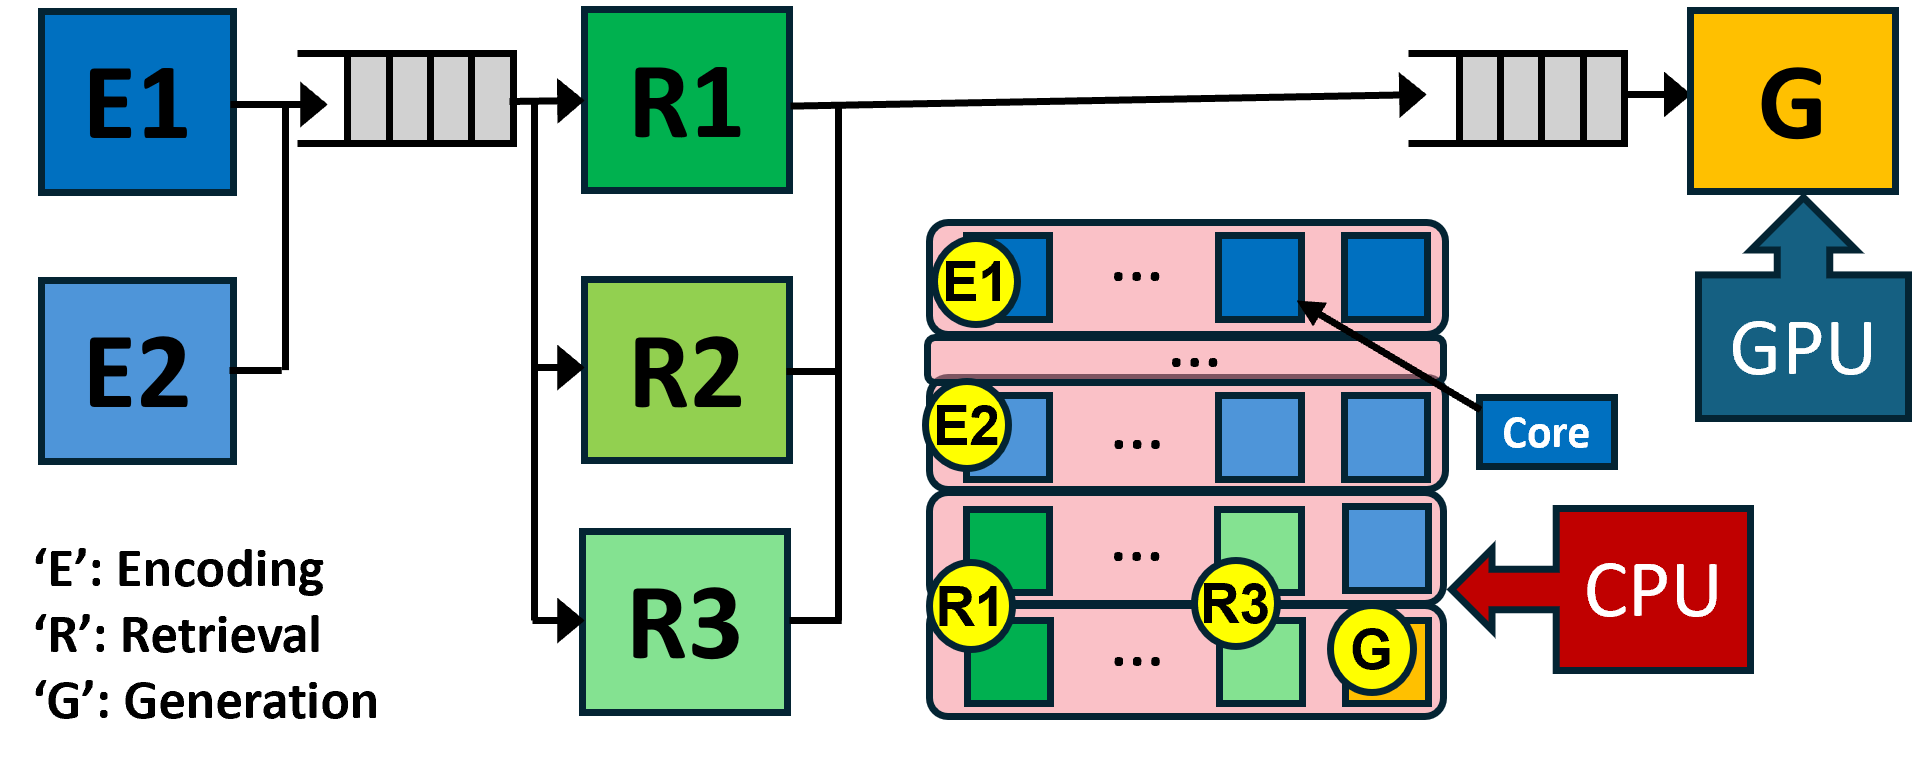
\includegraphics[width=1\linewidth]{diagrams/throughput_oriented_pipeline.png}
% \caption{Proposed pipeline for throughput-critical tasks having more number of parallel workers in the encode and retrieve stages to maximize the number of batches being processed in the pipeline.}
% \label{fig:throughput_oriented_pipeline} 
% \end{figure}

\noindent
%\textbf{Pipeline Overview.} 
\subsection{Pipeline Design Overview}
\label{subsec:pipeline_design}
Our pipeline comprises three stages: \emph{Encode}, \emph{Retrieve+Augment}, and \emph{Generate}. 
%The first stage, \emph{Encode}, takes the user query in natural language and transforms it into a higher-dimensional vector representation. The second stage, \emph{Retrieve+Augment}, uses these embeddings to perform a similarity search over the vector database, retrieving the top-$k$ relevant knowledge elements. The retrieved elements are then appended to the user query in a prompt format that can include directions for the Large Language Model (LLM), such as tonality (formal or casual), verbosity (concise or detailed), or accuracy (creative or pragmatic). Finally, the third stage, \emph{Generate}, takes this augmented query as input to the LLM in order to produce the final response.
%\noindent
%\textbf{Rationale for the Three-Stage Partitioning.}
The rationale for our three-stage design is based on our characterization study, which reveals that the \emph{Encode} stage typically involves computationally intensive floating-point and matrix operations, while the \emph{Retrieve} process is largely memory-bound, requiring searches through lists of indices. These two operations, if implemented together on the same CPU cores, can interfere with each other’s cache contents, causing higher miss latencies. By dedicating an \emph{exclusive} set of CPU cores to each stage (by specifying the core affinity to the process running), we exploit the reuse of model parameters and index data within those cores across batches without polluting caches and by containing the working set of that process within the private cache hierarchy of those cores. Consequently, we separate these stages from the conventional single \emph{retrieve} step often seen in RAG pipelines. 

Since the \emph{Augment} operation (\S\ref{sec:BG:Augmentation}) shares a working set similar to retrieval, we opt to merge \emph{Retrieve} and \emph{Augment} into a single stage. Although running retrieval and augmentation as distinct processes can, in theory, offer benefits in terms of cache isolation, the overhead of inter-process communication and synchronization often outweighs the gains. Therefore, \emph{Encode} and \emph{Retrieve+Augment} each run on a dedicated set of CPU cores, followed by the \emph{Generate} stage, ensuring efficient use of system resources at every step. 
%In our empirical study 
Separating out augment and retrieval stages, although brings cache hit benefits in their respective private caches, but suffers from synchronization and data transfer overheads across processes (resulting in latency increase of the two stages, up to 128 ms on average)\flag{Untraced: the 128\,ms augment-separation cost appears in no workbook tab and in no rebuttal sentence.}, overshadowing the benefits from cache hits.

Our design for an edge personal computing device targets two main types of user tasks: latency-critical and throughput-critical. A latency-critical task involves a virtual assistant that provides real-time insights, such as calendar summaries. A throughput-critical task focuses on generating recommendations for shopping, entertainment, or financial investments based on data from e-commerce, entertainment, and banking apps.
%An example of the latency critical task would be virtual personalized assistant conversing with the user with contextual knowledge like summarizing the calendar. A throughput critical task can be thought of providing user with recommendations about shopping, entertainment or financial investments, on the basis of their e-commerce, entertainment and banking app's data respectively.
The insights developed in the previous characterization study help us to use the multicore scalability of stages to our advantage to move towards a more balanced pipeline organization. As shown in \Cref{fig:latency_oriented_pipeline} and ~\Cref{fig:throughput_oriented_pipeline}, we introduce a resource-aware multi-width pipeline, where each stage can be executed in parallel on different numbers of CPU cores. Here, each `worker' is a process running independently on allocated cores capable of processing one batch at a time, and there can be a variable number of workers in each pipeline stage depending on the number of cores the CPU has and the type of latency/throughput need of the application. We develop different schemes to tackle the latency and throughput critical situations. For latency-critical workloads, we allocate maximum CPU cores to each worker in a single-width pipeline to minimize response time. For throughput-critical workloads, diverging from traditional pipeline design, we spawn multiple workers per stage with reduced per-worker core allocation, as shown in \Cref{fig:throughput_oriented_pipeline}. This configuration enables multiple request batches to be processed concurrently within the pipeline, compared to single-batch processing in the latency-optimized case (\Cref{subsec:resource-mapping}).

Our pipeline design differs from state-of-the-art methods as shown in \Cref{pipeline_comparison_schematic}. Existing pipelines typically perform encoding and retrieval on either CPUs or GPUs, followed by CPU-based augmentation and GPU-based generation~\cite{jin2024flashrag, jiang2024piperag, EdgeRAG}. FlashRAG and EdgeRAG utilize GPUs for encoding and generation, while performing retrieval on CPUs. PipeRAG, with certain optimizations, can disaggregate encoding and retrieval stages on CPUs followed by GPU-based generation, reducing pipeline bubbles compared to prior solutions. However, latency differences between stages and the synchronous pipeline nature do not fully eliminate bubbles. Our approach addresses this by orchestrating an asynchronous pipeline, where each stage receives compute resources proportional to its computational requirements.
%as discussed in the next section.

%%%%%%%%%%%%%%%%%%% ADDED BY CYAN %%%%%%%%%%%%%%%%%%%
% \noindent\textbf{Adaptive batching:} 
% The encoding stage is compute-bound and sensitive to core provisioning and batch size, whereas retrieval latency is dominated by I/O and memory operations, showing diminishing returns beyond moderate core counts (e.g., doubling from 8 to 16 cores; \Cref{Fig:latency_cores}). Thus, a fixed batch size and core allocation is suboptimal across different databases, workloads, and hardware. Using profiling insights from \Cref{sec:03Characterization}, we determine the ``sweet spot'' for batch size and core allocation per stage.
% Requests that exceed resource or SLO constraints are split into smaller quanta, processed asynchronously to avoid lock-step delays. This reduces I/O bottlenecks for large batches by completing retrievals faster and staggering memory accesses. Adaptive batching also mitigates GPU memory limits on personal compute devices by splitting oversized batches before scheduling them on the GPU. For GPU-bound jobs, the CPU process primarily launches kernels and collects data; we pin such lightweight tasks to E-cores, freeing P-cores for heavier stages.
%%%%%%%%%%%%%%%%%%%%%%%%%%%%%%%%%%%%%%%%%%%%%%%%%%%%%%%%%

\noindent\textbf{Adaptive batching:} 
%Insights from the previous characterization section reveal that the encoding and retrieval stages have different sensitivities with respect to both CPU core counts and batch sizes. 
The computationally bound encoding stage strongly correlates its latency with the amount of core provisioning and batch size. In contrast, that of the retrieval stage depends more heavily on the size of I/O and memory operations; as shown in ~\Cref{Fig:latency_cores}, doubling the core count from 8 to 16 generates diminishing benefits for latency. 
Thus, a one-size-fits-all approach to batch size and core allocation is not optimal across different databases, batch profiles, models, and hardware architectures. Instead, a more flexible and judicious compute allocation strategy is required, taking into account the specific operation, service-level objective (SLO) constraints, hardware details, and the RAG model itself. Leveraging the profiling results discussed in \Cref{sec:03Characterization}, we identify the “sweet spot” for batch size and core allocation for each stage.

% However, there are scenarios where the request size and SLO requirements require the execution of a batch larger than the provisioning allows. In such cases, the large batch is split into smaller, more efficient quanta, thus maximizing resource utilization while minimizing overall latency. To further streamline performance, these smaller quanta are processed asynchronously, reducing any lock-step synchronization overhead in the pipeline. Whenever a worker finds tasks in its input queue, it immediately begins to process a batch, even if another worker is momentarily a straggler. This approach particularly benefits large batch sizes, where the retrieval stage would otherwise incur substantial I/O overhead. By breaking up large I/O requests into multiple smaller quanta, we achieve two primary advantages: first, each retrieval operation has a quicker turnaround, allowing the batch to proceed to the next state sooner; and second, read requests are staggered over time, reducing the likelihood of saturating memory bandwidth.
However, some requests exceed the available provisioning for their batch size or SLO constraints. In such cases, we split large batches into smaller quanta, maximizing resource usage and minimizing overall latency. These quanta are processed asynchronously to avoid lock-step overhead: whenever a worker finds tasks in its input queue, it proceeds immediately, regardless of any straggling peers. This is especially beneficial for large batches, where the retrieval stage would otherwise suffer significant I/O overhead. By breaking large I/O requests into smaller chunks, individual retrievals complete faster,
%(accelerating the pipeline),
and the staggered read requests reduce the risk of saturating memory bandwidth. 

Since the memory capacity of the GPU in a typical personal computing platform is smaller, it is capable of generating responses for a limited number of prompts before it goes out of memory. Adaptive batching alleviates this bottleneck by breaking down the larger batch of requests for a GPU into smaller quanta and scheduling them. For the GPU bound jobs, typically the process running on a CPU acts as an agent to only launch kernels and collect the data back. 
%Since this process has a lightweight computational footprint and computations follow sporadic burst-like patterns, we preferably assign them E-cores, which are traditionally not used for computationally heavy-lifting applications.
Given their lightweight, bursty nature, these tasks are best scheduled on E-cores, which are typically reserved for non-intensive workloads.
\new{Generation latency depends on the intended prompt length. The mapper profiles $T_{G}$ across those lengths (\Cref{subsec:resource-mapping}), and adaptive batching creates memory-safe GPU quanta. Worker allocation is nonetheless static within a session, following the start-up amortization rationale of \Cref{sec:Design:Software}. Remapping cores at run time under context drift is a future extension.}

%Thus, we need a "scheduler" that serializes the requests going to the GPU for generation, making sure that the GPU is neither oversubscribed nor is it underutilized by small batches of queries where other batches are also ready and waiting to be executed on the GPU. This scheduler acts as an "agent" to launch kernels to the GPU with the minimum possible latency from the CPU side. Thus, we allocate a fixed core to this generation scheduling process. Since this process has a lightweight computational footprint and computations follow sporadic bursts like pattern, we preferably assign them E-cores, which are traditionally not used for computationally heavy-lifting applications.

% \begin{figure}
% \centering
% 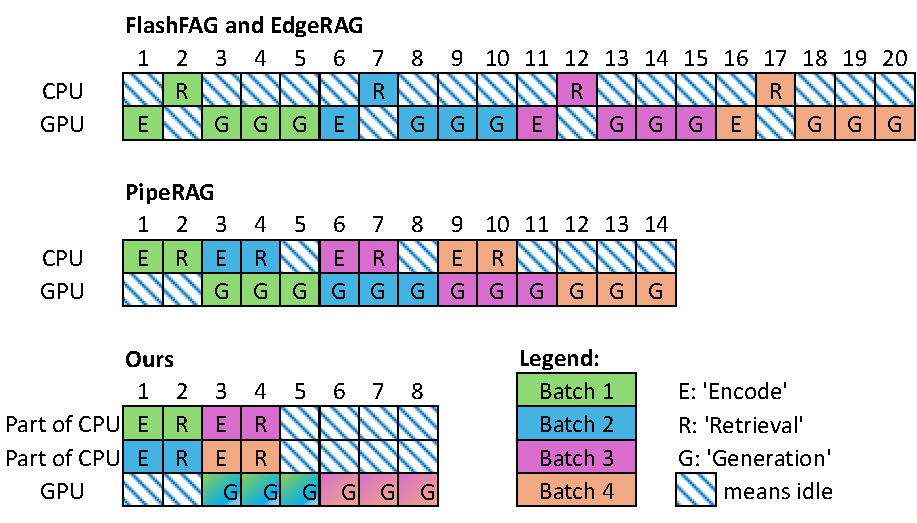
\includegraphics[width=1\columnwidth]{diagrams/pipeline_comparison_schematic.pdf}
% \caption{A example pipeline representation comparing prior works with our approach. Multiple batches are executed on the same hardware platform (comprising of CPU and GPU). X-axis represents the time steps and Y-axis shows the utilization of compute unit. Note that part of CPU means using a fraction of CPU cores for a specific stage.}
% \label{fig:pipeline_comparison_schematic} 
% %\vspace{-5mm}
% \end{figure}

\subsection{Resource Mapping}% for a Heterogeneous Pipeline}
\label{subsec:resource-mapping}

% Our design assigns the CPU-based stages (\emph{encoding, retrieval, and augmentation}) to CPU cores, while the \emph{generation} stage runs on a dedicated GPU. Most modern CPUs are equipped with different numbers of heterogeneous types of cores: P-cores (high throughput) and E-cores (energy efficient). Let $N_P$ and $N_E$ denote the number
% of P) and E cores, with $N = N_P + N_E$ total CPU cores. 
% Our design assigns the CPU-based stages (\emph{encoding and  retrieval+augmentation}) to CPU cores, while the \emph{generation} stage runs on a dedicated GPU. Many modern CPUs integrate \emph{performance cores (P-cores)} for high throughput and \emph{efficiency cores (E-cores)} for low power consumption. For modeling, let $N_{P}$ and $N_{E}$ be the numbers of P-cores and E-cores, respectively, such that the total number of CPU cores is $N = N_{P} + N_{E}$.
% Each CPU-bound stage--encoding ($E$) and retrieval+augmentation ($RA$)---is allocated $(x_s,y_s)$ P- and E-cores, where $s\in\{E,RA\}$.

% \noindent\textbf{Stage Profiling.}
% First, we measure $T_s(x,y)$, the latency of each stage $s$ on $x$ P-cores and $y$ E-cores, across feasible $(x,y)$ pairs. We also measure the GPU generation time $T_G$ for the desired prompt lengths or batch sizes. This profiling is repeated whenever the hardware configuration or LLM changes, keeping the system model-aware.

% \noindent\textbf{Latency-Critical Mapping.}
% For latency-sensitive use cases, the end-to-end time for a single batch is:
% $
% \mathrm{T}_{\mathrm{E2E}}(x_E,y_E,x_{RA},y_{RA}) 
% = T_E(x_E,y_E)\,+\,T_{RA}(x_{RA},y_{RA})\,+\,T_G,
% $
% under constraints $x_E + x_{RA}\le N_P$, $y_E + y_{RA}\le N_E$. We choose $(x_s,y_s)$ to minimize
% this sum or meet an SLO $L_{\max}$, often through a small grid search.

% \noindent\textbf{Throughput-Critical Mapping.}
% For sustained workloads, multiple workers $w_s$ can be launched per stage $s$, each using
% $(\tilde{x}_s,\tilde{y}_s)$ cores. The throughput per stage is
% $\mathrm{TH}_s = w_s / T_s(\tilde{x}_s,\tilde{y}_s)$,
% subject to $\sum_s w_s \tilde{x}_s \le N_P$ and $\sum_s w_s \tilde{y}_s \le N_E$. We then maximize
% the minimum throughput across $s$, ensuring that the GPU
% generation throughput is also balanced. Note that, this formulation for the mapping is generic and involves both P- and E-cores. For sake of simplicity, in our experiments, we have treated all the cores to be the same (i.e. $y = 0$). The proposed design can be extend into complex systems where the P- and E-cores vary in performance staggeringly.

Our design assigns the CPU--based stages, \emph{encoding} ($E$) and \emph{retrieval+augmentation} ($RA$), to CPU cores, while the \emph{generation} ($G$) stage runs on GPU. Modern CPUs often feature \emph{performance cores (P-cores)} for high throughput and \emph{efficiency cores (E-cores)} for low power usage. We denote their counts by $N_{P}$ and $N_{E}$, respectively, so that $N = N_{P} + N_{E}$ is the total number of CPU cores.
%\noindent\textbf{Stage Profiling.}
We profile the latency $T_{s}(x,y)$ of each CPU--bound stage $s \in \{E,RA\}$ under different allocations of $x$ P-cores and $y$ E-cores. For generation, we measure $T_{G}$ given the intended prompt lengths or batch sizes. These profiles are re-measured whenever the hardware configuration or LLM changes, keeping the system \emph{model-aware}.
%\noindent\textbf{Latency-Critical Mapping.}
For latency-sensitive batches, the end-to-end time is given by
$T_{\mathrm{E2E}}(x_E,y_E,\ x_{RA},y_{RA}) = T_E(x_E,y_E)\;+\;T_{RA}(x_{RA},y_{RA})\;+\;T_G,$
subject to $x_E + x_{RA} \le N_{P}$ and $y_E + y_{RA} \le N_{E}$. One can choose $(x_s,y_s)$ per stage $s\in\{E,RA\}$ to minimize $T_{\mathrm{E2E}}$ or meet a latency SLO $L_{\max}$, typically by using a small grid search.
%\noindent\textbf{Throughput-Critical Mapping.}
For sustained workloads, each CPU--bound stage $s\in\{E,RA\}$ may run $w_{s}$ workers, each allocated $(\tilde{x}_s,\tilde{y}_s)$ P- and E-cores. The throughput is: 
$
  \mathrm{TH}_s
  \;=\;
  \frac{w_{s}}{T_{s}(\tilde{x}_s,\tilde{y}_s)},
$
subject to $\sum_{s} w_{s}\,\tilde{x}_s \;\le\; N_{P}$ and 
$\sum_{s} w_{s}\,\tilde{y}_s \;\le\; N_{E}$. We then maximize the minimum throughput across all stages %(including GPU $G$) 
for balanced performance. In our experiments, we treat all CPU cores uniformly (i.e.,\ $y=0$), but this design naturally extends to systems where P- and E-cores differ in performance. 
% \red{
% Using the above equations to our desktop-grade CPU platforms, we find the optimal core allocation strategy for latency critical application to be \textbf{E:8, R:22, G:1} and the remaining one core for the scheduler to run on. With mapper identified configuration, the our three stage pipeline (\texttt{DB = 2\,M; BS=8}) takes $1.178\,s$ $\langle E=0.21, RA=0.78\rangle$, whereas the standard four stage piepline takes $1.448\,s$ $\langle E=0.192, R=0.761, A=0.104\rangle$, which is much better than na\'ive allocation approach which takes $13.22\,s$ (in both cases the \textbf{G} stage is ignored as it takes the same time). The proposed three stage pipeline provides an $\approx 22\%$ better performance over the four stage approach thanks to less scheduler overheads.
% }

As an example, applying the above equations to our desktop-grade CPU platform, we determine the optimal core allocation strategy for the latency-critical application to be \textbf{E:8, RA:22, G:1}\footnote{With Jetson at a 15W power budget (see \Cref{subsec:implementation}), we get 4 cores to work with of which 2 are used for \textbf{E}, 1 for \textbf{RA} and 1 for \textbf{G} and scheduler.}, with the remaining single core dedicated to the scheduler. Under this mapper-identified configuration, our proposed three-stage pipeline (\texttt{for DB=2\,M; BS=8}) results in an execution time of $1.178\,\mathrm{s}$ with a stage-wise breakdown of $\langle$E=0.21s,\, RA=0.78s$\rangle$ and a scheduler overhead of 0.188s. In comparison, the standard four-stage pipeline requires $1.448\,\mathrm{s}$ with the breakdown $\langle$E=0.192s,\,R=0.761s,\,A=0.104s$\rangle$ along with scheduler overhead of 0.391s. Both configurations ignore the \textbf{G} stage, as its execution time remains constant. 
Notably, our three-stage pipeline delivers a \new{$1.23\times$} improvement over the four-stage approach, primarily due to the reduced scheduler overhead. This performance is also significantly better than the naïve allocation strategy, which requires $9.5\,\mathrm{s}$ ($8.06\times$) for similar CPU execution.


\noindent\textbf{Multi-Worker Duplication:}
Although dedicating more cores can reduce latency for one worker, we often scale \emph{width} by creating additional workers on fewer cores, thereby feeding the pipeline more batches and avoiding CPU underutilization. In practice, the generation stage is often slowest; 
however, limiting encode/retrieve to modest core counts often yields better overall throughput, since more workers can run in parallel. Duplication can inflate memory use if each worker loads its own model or index; therefore, optimizations (in \Cref{sec:Design:Software}) to share these large data structures between processes.
\red{For instance, as depicted in \Cref{fig:latency_oriented_pipeline}, allocating 8 cores per worker for stage E, 22 cores per worker for stage RA, and 1 core per worker for stage G achieves a latency of 4.898s. In contrast, the configuration in \Cref{fig:throughput_oriented_pipeline} with 4 cores per worker for stage E (2 workers), 6 cores per worker for stage RA (3 workers), and 1 core per worker for stage G (1 worker), yields a latency of 5.347s while serving 3× the number of requests on  Intel i9-14900K platform paired with RTX 4090 GPU.}

\noindent\textbf{Adaptive Mapping:}
Once $T_s(x,y)$ and $T_G$ have been profiled, we solve either a latency-oriented or a throughput-oriented formulation under the same CPU constraints. We then \emph{pin} each stage (or worker group) to its allocated P- and E-cores. Re-running this procedure on a new device or LLM keeps the pipeline \emph{hardware-aware} as well as {\em model-aware,} consistently aligned with SLO targets.
%Figure~\ref{fig:pipeline_comparison_schematic} shows how the proposed pipeline compares with the state-of-the-art RAG pipelines. 
The benefits of the proposed mapping are further discussed in \Cref{sec:additionalInsights}. 
%We can observe that we maximize the execution time overlap possibility across multiple CPU cores, dedicated towards same/multiple batches, with GPU execution time, helping us improve the overall execution time along with throughput.
%\rishabh{refer to Figure~\ref{fig:pipeline_comparison_schematic} in this subsection}


% \subsection{Resource Mapping for Heterogeneous Pipeline}% CPU-GPU Pipelines}
% \label{subsec:resource-mapping}
% In our design, the CPU-based stages (\emph{encoding, retrieval, and augmentation}) are executed on heterogeneous CPU cores, while the final \emph{generation} stage is offloaded to a dedicated GPU.
% We let $N_P$ and $N_E$ denote the number of performance (P) and efficiency (E) cores, respectively, with $N = N_P + N_E$ as the total number of CPU cores. Each of the three CPU-bound stages (\emph{encoding (E), retrieval+augmentation (RA)}) may receive $(x_s, y_s)$ P-cores and E-cores respectively, where $s \in \{E,RA\}$.


% \noindent\textbf{Stage Profiling.}
% We begin by empirically measuring $T_s(x, y)$, the processing time of each stage $s$ on $x$ P-cores
% and $y$ E-cores, over a grid of feasible $(x,y)$ pairs. This profiling is performed at system
% initialization or whenever the hardware configuration or LLM changes (e.g., switching to a larger
% model or deploying on a new platform). We similarly measure the GPU-based generation time, $T_G$,
% for relevant batch sizes and prompt lengths.
% %(see Section~\ref{sec:gpu-latency} for further details).


% \noindent\textbf{Latency-Critical Mapping.}
% In latency-sensitive scenarios, we define the end-to-end time for a single batch as
% \begin{equation}
% \begin{aligned}
% \mathrm{Time}_{\mathrm{E2E}}(x_E, y_E, x_{RA}, y_{RA}) 
% &= T_E(x_E,y_E) \;+\; T_{RA}(x_{RA},y_{RA}) + T_G,%\\
% %&\quad + T_A(x_A,y_A) + T_G,
% \end{aligned}
% \label{eq:latency}
% \end{equation}
% where the constraint
% \begin{equation}
% \label{eq:hetero-constraints}
% x_E + x_{RA} \;\le\; N_P, 
% \quad
% y_E + y_{RA} \;\le\; N_E,
% \quad
% x_s,y_s \;\in \mathbb{N}_0,
% \end{equation}
% must be satisfied. We then minimize the total latency or ensure it meets an SLO $L_\mathrm{max}$:
% \begin{equation}
% \label{eq:LC-objective}
% \min_{\substack{x_s,y_s}} \, \mathrm{Time}_{\mathrm{E2E}}(x_E, y_E, x_{RA}, y_{RA})
% \quad \text{subject to} \quad \eqref{eq:hetero-constraints}.
% \end{equation}
% In practice, we conduct a small integer grid search for $(x_s,y_s)$ that yields feasible per-batch
% latency under $L_\mathrm{max}$ with minimal resource usage, or directly solve~\eqref{eq:LC-objective}.


% \noindent\textbf{Throughput-Critical Mapping.}
% For a continuous stream of requests, we adopt multiple workers for each CPU stage, $w_s$, each
% assigned $(\tilde{x}_s,\tilde{y}_s)$ P- and E-cores. The throughput of stage $s$ becomes
% $\mathrm{TH}_s = w_s / T_s(\tilde{x}_s,\tilde{y}_s)$. Hence, the total P-cores and E-cores consumed
% are $\sum_s w_s \,\tilde{x}_s \le N_P$ and $\sum_s w_s \,\tilde{y}_s \le N_E$, respectively, leading
% to:
% \begin{equation}
% \begin{aligned}
% \max_{\substack{w_s,\tilde{x}_s,\tilde{y}_s}} \;\;
% \min_{s \in \{E,RA\}} 
% \biggl[\tfrac{w_s}{T_s(\tilde{x}_s,\tilde{y}_s)}\biggr]\\
% \text{subject to}
% \sum_s w_s \,\tilde{x}_s &\le N_P, \quad
% \sum_s w_s \,\tilde{y}_s \le N_E.
% \end{aligned}
% \label{eq:TC-objective}
% \end{equation}

% The GPU-based generation time is measured separately as $T_G$; we typically ensure that its 
% effective throughput matches or exceeds the CPU stages for balance.

% As we see diminishing impact of provisioning more cores on latency improvement, for throughput critical applications we hold back on provisioning more cores to the same worker stage and create a duplicate set of worker doing the same operation increasing the pipeline width. Each individual stage now experiences increase in latency within tolerable range but ends up supplying more work to the succeeding stage making sure the stage idleness is minimized. In case of our pipeline construction, for a batch size as reasonable as 4 requests at a time, we observe that the latency of generation stage is more than its preceeding retrieval+augmentation stage which is in turn more than the latency of encoding stage. In nutshell, as we move forward in the pipeline, the latency typically increases for the stages. This is interesting to note that it makes sure that for a steady stream of requests, the successive stage is never gated by the execution time of the prior stage. In essence the pipeline bubbles are not formed in this style of execution. We do not negate the possibility of work piling up for the last GPU bound generation stage because of the inability to duplicate its worker because of the existance of a single GPU only. But this way of execution makes sure that we are only limited by the hardware resource and not by the pipeline orchestration.

% Since each worker is a process working on a set of CPU cores, the duplication of these software workers run the downside of loading duplicate models and data which is redundant. The operations like encode and retrieval load models and large indices respectively into the main memory which when duplicated can saturate the main memory very fast without bringing any benefits. That is why we propose set of software optimizations to complement the pipeline orchestration without suffering the disadvantages of worker duplication.


% \noindent\textbf{Adaptive Mapping.}
% Upon collecting profiling data and specifying whether the focus is latency-sensitive (with or without 
% an explicit $L_{\max}$) or throughput-oriented, we solve the appropriate objective~\eqref{eq:LC-objective}
% or~\eqref{eq:TC-objective} under the constraints~\eqref{eq:hetero-constraints} or its multi-worker
% variant. The resulting integer solution directly indicates how many P-cores and E-cores to allocate 
% to each stage, or to each worker group if running multiple pipeline instances. Finally, we \emph{pin}
% threads for each stage to these assigned CPU cores.
% By re-running this procedure on a new device or under a different LLM, we can update our stage
% latencies $T_s$ and generation time $T_G$ to reflect the changed setting, then re-solve the same
% formulation with minimal user intervention. This \emph{quick-profiling} and \emph{adaptation} step ensures that the pipeline remains hardware-aware
% (\emph{e.g.}, balancing distinct P/E cores), model-aware (\emph{e.g.}, adjusting for slower or faster
% encoders), and compliant with the desired target (either an explicit SLO or a throughput
% goal).

%\begin{algorithm}[t]
\caption{Quick-Profiling and Adaptation}
\label{alg:profiling}
\begin{algorithmic}[1]
\State \textbf{Input:} \# of P-cores $N_P$, E-cores $N_E$, set of stage-latency tests,
       objective type (latency or throughput), optional SLO $L_{\max}$.
\State \textbf{Output:} A feasible mapping $(x_s,y_s)$ (or multi-worker $\tilde{x}_s,\tilde{y}_s,w_s$).

\State \textbf{Step\,1.} Profile each CPU stage $s$ to measure $T_s(x,y)$ on $(x,y)$ pairs and record $T_G$.
\State \textbf{Step\,2.} Determine whether to solve for latency-critical \eqref{eq:LC-objective} 
      or throughput-critical \eqref{eq:TC-objective} demands. 
\State \textbf{Step\,3.} Solve the respective integer problem subject to $x_s,y_s \ge 0$ and
      $x_E+x_{RA}\ \le N_P$, $\,y_E+y_{RA} \le N_E$ (or the multi-worker constraints).
\State \textbf{Step\,4.} Pin CPU threads for each stage to the chosen (P,\,E) cores and confirm
      end-to-end pipeline metrics meet the target SLO or throughput objective.
\end{algorithmic}
\end{algorithm}


%\subsection{Caching Policies}
% A. Multiple types of caching - 
% 0. Model caching. We keep the encoding model cached. using memap/shared memory (python), so that when we assign multiple workers to work on the same model, they dont load model over and over again and createthe local copies. Reduces memcopy significatly and greatly increases performance.   
% 1. Query caching: Cache the embedding of the query after the encoding. So, if the same/smilar embedding comes then not do the encoding, and straight go to the retrieval stage onwards (skips embedding)
% 2. Retrieval cachig: Cache the top-k retrieval results of the query agains the query embedding vector as a dictonary. So, if the same/ similar query comes, then we do not have to perform either the embedding or the retrieval. Further more, if there are hierarchical clustering (FLAT IVF kind) based indexing, and entire cluster can be cached, then the lookup for the etire cluster  can be skipped from the storage. So, we skip/skim the retrieval stage and go to generate. 
% 3. Dupilcate Query Caching: We cache the query embedding against the geeration results. If, by chance, a query is repeated, and we find both the query and generation to be cached, we can skip the generation as well and returning the previous results.
% B. Everywhere we use LRU caching policy. The caching is not new, and prior works lik CAG (Don’t Do RAG: When Cache-Augmented Generation is All You Need for Knowledge Tasks) have shown effeciveness of the caching policy. However, we are emplying it in the mobile devices with stricter constraints. 
% C. Explain how the data flow with caching is working. 

\subsection{System and Software Optimizations}
\label{sec:Design:Software}
Our pipeline orchestration lies in the allocation of the available CPU cores and assigning them to workers (processes running the stage) judiciously. For applications that are throughput critical, we make redundant workers to increase the width of the software pipeline. On the other hand, for latency-critical applications, we allocate maximal CPU cores to reap the most benefit in latency. We observe a few inefficiencies in the naive orchestration of this pipeline. First, the worker initialization process that comprises configuring the threads, loading the encoding model, and fetching the indices from the disk to the main memory is expensive. Having multiple such workers leads to redundant copies of the same data. Second, breaking down the requests of larger sizes into smaller quanta leads to creation of multiple batches, which in essence lead to multiple start-up costs that can impact the throughput of the system. In order to address these inefficiencies, we implement several orchestration optimizations:

\noindent\textbf{Shared data access:} Multiple workers in encoding and retrieval stages exhibit a high reuse of the same model and indices, respectively. A naive way of execution would load these data privately to the respective processes and access them. We implemented model weight sharing across processes through a shared memory mechanism, eliminating redundant copies of large model parameters, which saves us the time to fetch the same. 
%Similarly, our memory-mapped indices allow multiple retrieval workers to access the same index from disk without duplicating it in memory, reducing the memory footprint.

\noindent\textbf{Memory mapped indices:} This approach maps the index file directly to the virtual memory space without completely loading it into RAM. The operating system handles paging as needed, bringing only the accessed portions to physical memory. This enables our system to work with indices that are significantly larger than available RAM while maintaining performance through OS-level caching mechanisms. 
%For large knowledge bases ($> 1Mil$ vectors), this reduces initialization time from minutes to seconds and enables operation on memory-constrained systems.

\noindent\textbf{Start-up costs:} Launching workers per arrived batch leads to multiple start-up costs compared to the actual processing time. Since our classification (latency and throughput critical) remains static throughout the request, the number of workers can be fixed apriori and need not change during the execution of the successive batches. Separating out the worker initialization from the task execution causes these costly start-up operations to happen only once before any requests are even launched.  It might impact the execution time if the nature of the application changes on the fly. 
%from throughput sensitive to latency sensitive or vice versa.
But this is a design decision that we expect the user to make that presents a reasonable tradeoff in most real-world scenarios, where application requirements tend to remain consistent throughout an operational session.

% \subsection{Caching Policies}
% \label{sec:Design:Caching}
% Caching plays a vital role in reducing redundant computations and memory transfers in our RAG pipeline, especially on resource-limited devices. By selectively storing intermediate results in fast-access caches, we minimize repeated operations such as retrieval lookups, which consists of costly vector similarity searches, thereby improving both latency and throughput. Also, for our target deployment on edge devices, where the context of the successive queries largely remains the same, we believe caching is a natural progression in the set of design choices. This section outlines our caching strategies, drawing on key insights from prior work on cache-augmented generation~\cite{chan2024don} and adapting them for edge platforms with stricter memory and power constraints.

% \begin{figure}
% \centering
% 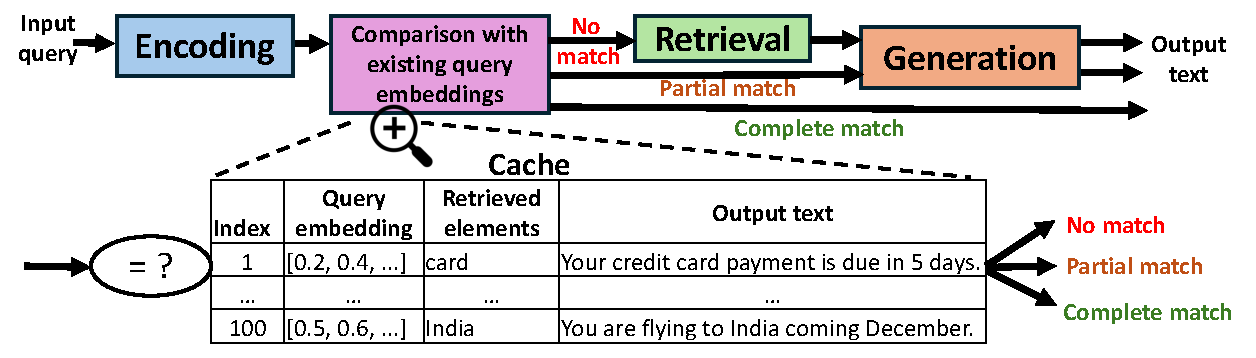
\includegraphics[width=1\columnwidth]{diagrams/caching_design.pdf}
% \caption{{Logical view of our caching scheme.}}
% \label{fig:caching_design} 
% \vspace{-10pt}
% \end{figure}

% A central feature of our design is \textit{model caching}, where we keep the encoding model resident in the main memory (or a shared memory region) across multiple parallel workers. Rather than loading the encoder separately for each worker, we store it once in a dedicated memory map. This approach eliminates redundant memory copies and shortens the model loading time, as the model weights need not be re-initialized on each query. 
% %Through this shared model cache, GPU (or CPU) resources are instantly accessible to multiple worker threads in turn, alleviating bottlenecks that arise from frequent load/unload cycles.

% The edge computation use cases are typically dependent on the user's interaction with the device, where patterns can be found about the nature, frequency, and the likelihood of the queries. Such patterns are even more vital in RAG use cases, where the database is local to an user and any set of queries are serviced only by the help of limited knowledge bases. The need to reuse the previously fetched/generated data becomes even more important as the likelihood of variation of the output given the same input is minimal with the added advantage of saving power. Thus, we propose two types of data caching schemes as depicted in \Cref{fig:caching_design}.

% \noindent\textbf{Similarity/Partial match based retrieval caching:} In this scheme, we recognize semantic similarity between queries and leverage the previously computed results to service the future queries provided the semantic similarity falls in an agreeable range. The system stores each query embedding along with its retrieved documents. When a new query arrives, its embedding is compared against cached embeddings using cosine similarity. If the similarity exceeds a configurable threshold (e.g., 90\%), the system reuses the previously retrieved documents, bypassing only the retrieval phase, while still performing the generation step. \red{This threshold, supported by recent research~\cite{simThreshold, simThreshold1, simThreshold2, simThreshold3}, is carefully chosen to preserve the factual accuracy of responses while improving latency. Retrieval relies on exact flat-indexing to maximize recall, ensuring that semantic similarity does not come at the cost of correctness. Each cache entry includes a user-configurable time-to-live (TTL), typically a few minutes, during which the entry is considered valid. Both the similarity threshold and TTL are tunable, allowing fine-grained control based on system requirements.} By using the prior similar query's retrieved elements, the RAG pipeline eliminates the most latency incurring operation, while still being able to cater to the newly arriving query's nuances through a fresh generation.  

% \noindent\textbf{Exact/Complete match caching:} The basis of this scheme is to detect the repeated queries coming to the pipeline over time. When a new query arrives, the encoding model generates embedding and does a cache lookup to find out the most similar previously serviced query. In case of exact match, the subsequent stages in the pipeline are bypassed, and the final generated output is given to the user. The primary assumption is that the state of the vector database since the service of the prior query to the arrival of this new query has not changed. Given that we we keep track of the \textit{time to live} of each of these cache entries, which is typically a few minutes, it is highly likely that the vector database remains the same. This caching avoids any repeated decoding overhead and is valuable when certain prompts are repeated verbatim during a user session.
%We further employ \textit{query caching}, where embeddings of previously encoded queries are stored in an in-memory key-value structure keyed by the textual form of the query (or a hashed representation). If an incoming query matches a cached entry, the corresponding embedding is retrieved immediately instead of performing encoding again. On personal computing devices, user queries often recur or share common substrings, so this caching technique substantially reduces repeated encoding overhead. In our system, an additional similarity check can also be enabled: if an incoming query is semantically close to a cached query embedding, we reuse the cached encoding. This is especially beneficial when the system observes bursts of requests on semantically similar prompts.
%In terms of \textit{retrieval caching}, we store not only the query embeddings but also the top-$k$ retrieval results for each query. When an identical or near-duplicate query arrives, the retrieval stage can be bypassed altogether, with the previous top-$k$ items used directly. Depending on the nature of the underlying index (e.g., a flat or IVF-based structure), we may also cache entire clusters or neighborhoods within the vector space. This coarse-grained clustering cache is particularly effective if multiple incoming queries fall into the same region of the embedding space. In such scenarios, the index lookup can be short-circuited, and the cached cluster is handed directly to the generate stage, thus skipping both embedding and retrieval.
%Beyond retrieval caching, we also implement \textit{duplicate query caching} at the generation stage. Here, we record the final output for queries whose retrieval sets and augmented prompts are identical. If the same query embedding and top-$k$ retrieval items reappear, we can return the previously generated text immediately. This final-level caching avoids any repeated decoding overhead and proves valuable when certain high-frequency prompts are repeated verbatim during a user session.
%Across these cache layers, w
%We adopt an LRU replacement policy to manage limited cache space and ensure that the most frequently accessed or most recently used results remain resident. 
%Our policy choice is motivated by findings from prior work~\cite{chan2024don} indicating that simple caching can be highly effective, even on mobile-class hardware. 
%We aggressively tune cache sizes to balance memory footprint with cache hit rates, placing particular emphasis on query-embedding caches in order to prune the computationally heavy encoding stage.

%Figure~\ref{fig:caching_design} illustrates our data flow with caching enabled. When a user query arrives, the system first checks the query cache for a matching or similar embedding. If found, the subsequent retrieval results might already be stored, allowing an immediate fetch to pass along to the augmentation step. Otherwise, the system encodes the query, stores the result, and performs a retrieval, optionally caching top-$k$ results for future reuse. Finally, if the query embedding plus top-$k$ results appear in the generation cache, the final text is returned right away. Otherwise, the generation step runs, and the new output is cached for potential queries later.

%By combining multiple levels of caching, the system effectively reduces repeated work across all RAG stages. This is of particular benefit on smaller, energy-constrained devices where model loading and data movement are prime bottlenecks. Evaluations show that even a modest LRU cache can significantly cut down on encoding overhead and retrieval latency. Hence, caching in all these forms serves as a practical cornerstone of our RAG design, maintaining performance on par with server-class methods yet fitting within the tight resource envelopes found on modern consumer devices.
%%%%%%%%%% %%%%%%%%%% %%%%%%%%%% %%%%%%%%%% 
% Text matter end

%%%%%%%%%%%%%%%%%%%%%%%%%%%%%%%%%%%%%%%%%%%%%%%%%%%%%%
 \begin{figure*} 
    \subfloat[E2E latency of \design{} in RTX4090.]
    {%
     % CR-REPLACED: 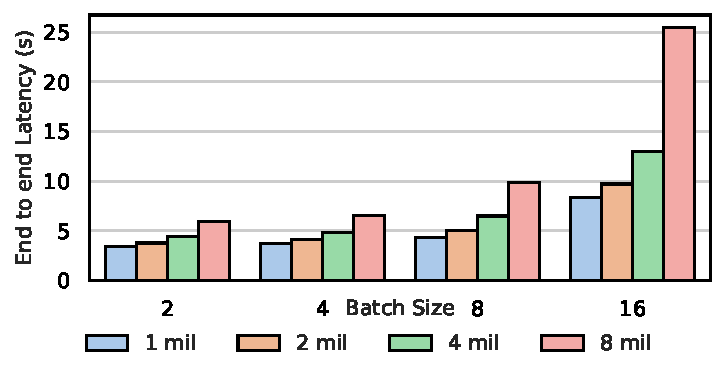
\includegraphics[clip,width=0.32\linewidth]{Figs/4090LatencyOurs.pdf}%
     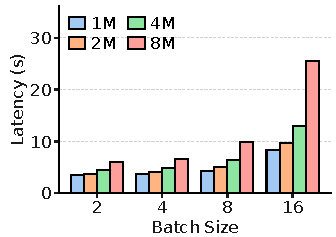
\includegraphics[clip,width=0.32\linewidth]{Figs/cr/4090LatencyOurs.pdf}%
    \label{Fig:OurLatencyE2E4090}
    }
    \hfill
    \subfloat[Speedup: \design{} vs EdgeRAG~\cite{EdgeRAG}.]
    {%
     % CR-REPLACED: 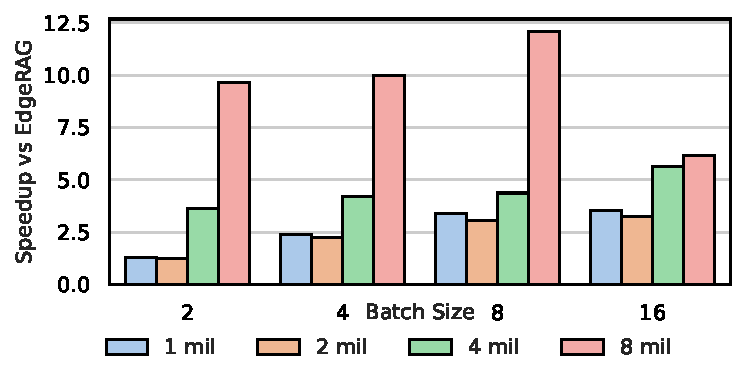
\includegraphics[clip,width=0.32\linewidth]{Figs/4090speedupEdgeRAG.pdf}%
     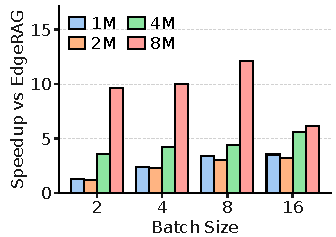
\includegraphics[clip,width=0.32\linewidth]{Figs/cr/4090speedupEdgeRAG.pdf}%
    \label{Fig:Lat-vs-EdgeRAG}
    }
    \hfill    
    \subfloat[Speedup: \design{} vs FlashRAG~\cite{jin2024flashrag}.]
    {%
     % CR-REPLACED: 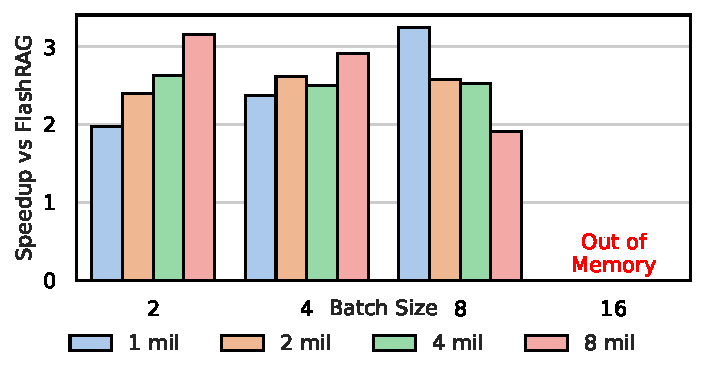
\includegraphics[clip,width=0.32\linewidth]{Figs/4090speedupFlashRAG.pdf}
     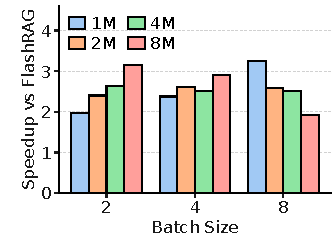
\includegraphics[clip,width=0.32\linewidth]{Figs/cr/4090speedupFlashRAG.pdf}
    \label{Fig:Lat-vs-FlashRAG}
    }
    
    \subfloat[Speedup: \design{} vs PipeRAG~\cite{jiang2024piperag}.]
    {%
    % CR-REPLACED: 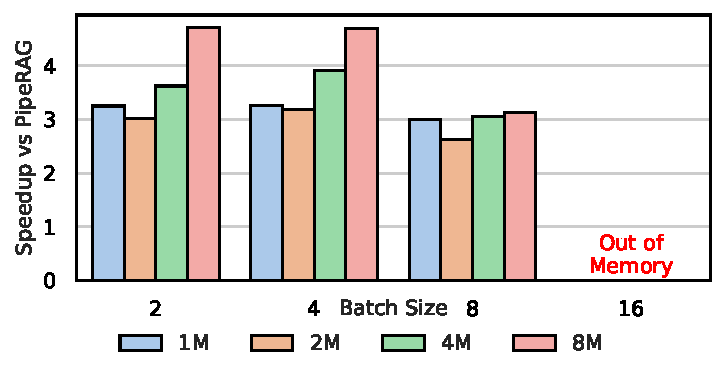
\includegraphics[clip,width=0.32\linewidth]{Figs/4090speedupPipeRAG.pdf}%
    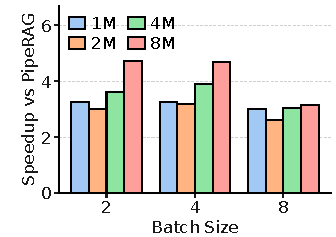
\includegraphics[clip,width=0.32\linewidth]{Figs/cr/4090speedupPipeRAG.pdf}%
    \label{Fig:Lat-vs-PipeRAG}
    }
    \hfill
    \subfloat[E2E latency of \design{} in RTX 4080]
    {%
    % CR-REPLACED: 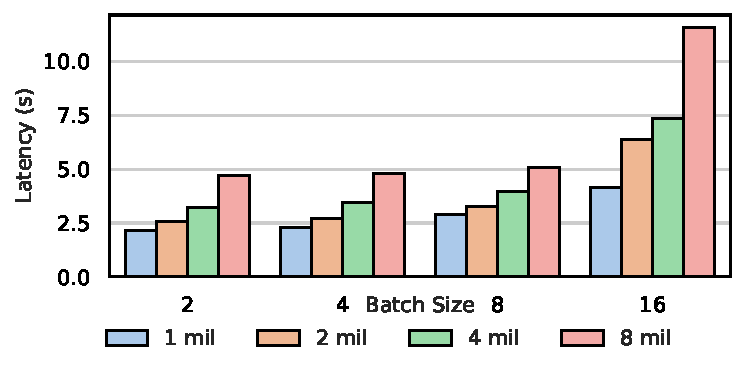
\includegraphics[clip,width=0.32\linewidth]{Figs/4080Latency_MaestroRAG.pdf}%
    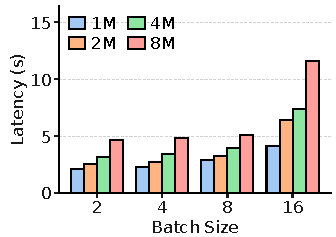
\includegraphics[clip,width=0.32\linewidth]{Figs/cr/4080Latency_MaestroRAG.pdf}%
    \label{Fig:4080Latency_Ours}
    }
    \hfill
    \subfloat[Speedup: \design{} vs other baselines.]
    {%
    % CR-REPLACED: 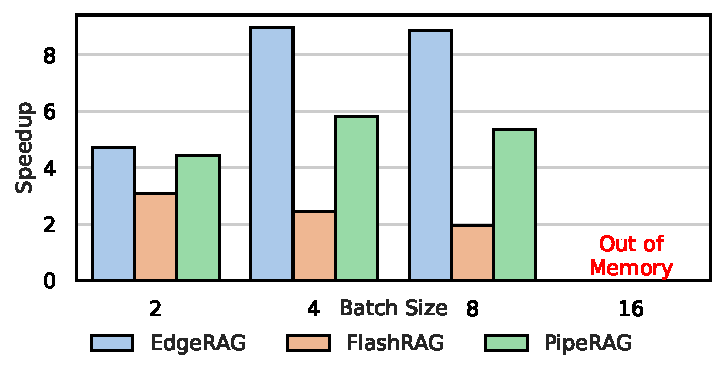
\includegraphics[clip,width=0.32\linewidth]{Figs/4080Speedup_Merged.pdf}%
    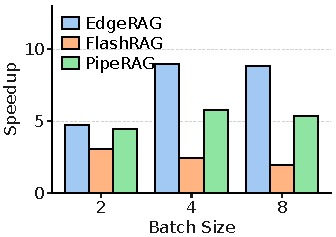
\includegraphics[clip,width=0.32\linewidth]{Figs/cr/4080Speedup_Merged.pdf}%
    \label{Fig:4080Speedup_Merged}
    }
    \caption{Speedup of \design{} relative to state-of-the-art RAG frameworks on consumer-grade systems with RTX 4090 (a--d) and RTX 4080 (e--f) GPU. 
    %MaestroRAG delivers speedups of up to $\approx 12.5\times$. 
    \new{The design elements evaluated here are described in \Cref{subsec:pipeline_design}, \Cref{subsec:resource-mapping}, and \Cref{sec:Design:Software}.}
    Caching was disabled during all evaluations to emulate random query patterns that lack spatio-temporal locality, representing a worst-case scenario commonly observed when extending from personal devices to large-scale serving frameworks. For MaestroRAG, we deploy one worker per pipeline stage with $\langle$\textbf{8}, \textbf{22}, and \textbf{1}$\rangle$ cores for the $\langle$\textbf{E}, \textbf{RA}, and \textbf{G}$\rangle$ stages, respectively. The \textbf{G} stage's allocated core is responsible for launching generation workers on the GPU and collecting results, while the system scheduler runs on the remaining available core.
    }
    %Caching functionality is deliberately disabled throughout the evaluation to model random query patterns characterized by the absence of spatio-temporal locality that can be extended from personal compute devices to serving frameworks.}
    %\fixme{Cyan: Change caption.1. pipelined orchestration, 2. heterogeneous resource mapping 3. adaptive batching with software optimizations}}

    %\vspace{-10pt}
    \label{Fig:Lat-All-4090}  
\end{figure*}
%%%%%%%%%%%%%%%%%%%%%%%%%%%%%%%%%%%%%%%%%%%%%%%%%%%%%%